\documentclass[a4paper, 11pt]{article}
\usepackage{comment} % enables the use of multi-line comments (\ifx \fi) 
\usepackage{lipsum} %This package just generates Lorem Ipsum filler text. 
\usepackage{fullpage} % changes the margin
\usepackage[a4paper, total={7in, 10in}]{geometry}
\usepackage[fleqn]{amsmath}
\usepackage{amssymb,amsthm}  % assumes amsmath package installed
\newtheorem{theorem}{Theorem}
\newtheorem{corollary}{Corollary}
\usepackage{graphicx}
\usepackage{caption}
\usepackage{bm}

% \usepackage[pdftex]{graphicx}
\usepackage{tikz}
\usetikzlibrary{arrows}
\usepackage{verbatim}
\usepackage[numbered]{mcode}
\usepackage{float}
\usepackage{tikz}
    \usetikzlibrary{shapes,arrows}
    \usetikzlibrary{arrows,calc,positioning}

    \tikzset{
        block/.style = {draw, rectangle,
            minimum height=1cm,
            minimum width=1.5cm},
        input/.style = {coordinate,node distance=1cm},
        output/.style = {coordinate,node distance=4cm},
        arrow/.style={draw, -latex,node distance=2cm},
        pinstyle/.style = {pin edge={latex-, black,node distance=2cm}},
        sum/.style = {draw, circle, node distance=1cm},
    }
\usepackage{xcolor}
\usepackage{mdframed}
\usepackage[shortlabels]{enumitem}
\usepackage{indentfirst}
\usepackage{hyperref}
\usepackage{CJKutf8}
\usepackage{url}

\renewcommand{\thesubsection}{\thesection.\alph{subsection}}

\newenvironment{problem}[2][Q]
    { \begin{mdframed}[backgroundcolor=gray!20] \textbf{#1 #2} \\}
    {  \end{mdframed}}

% Define solution environment
\newenvironment{solution}
    {\textit{Solution:}}
    {}

\renewcommand{\qed}{\quad\qedsymbol}
%%%%%%%%%%%%%%%%%%%%%%%%%%%%%%%%%%%%%%%%%%%%%%%%%%%%%%%%%%%%%%%%%%%%%%%%%%%%%%%%%%%%%%%%%%%%%%%%%%%%%%%%%%%%%%%%%%%%%%%%%%%%%%%%%%%%%%%%
\begin{document}
\begin{CJK}{UTF8}{gbsn}
%Header-Make sure you update this information!!!!
\noindent
%%%%%%%%%%%%%%%%%%%%%%%%%%%%%%%%%%%%%%%%%%%%%%%%%%%%%%%%%%%%%%%%%%%%%%%%%%%%%%%%%%%%%%%%%%%%%%%%%%%%%%%%%%%%%%%%%%%%%%%%%%%%%%%%%%%%%%%%
\large\textbf{课程: 人工智能} \hfill \textbf{作业 4}   \\
北航软件学院 \\
\normalsize 学期: 2025,春季\hfill 提交截止时间:  2025年6月21日, 11:59 PM \\
\noindent\rule{7in}{2.8pt}
\textbf{提醒注意:}
\begin{itemize}
\item 本次作业发布于2025年5月30日,截止于2025年6月21日。
\item 作业一分为三部分:问答题、实训题、以及实训题报告
\begin{itemize}
    \item 问答题答案可以手写并扫描,或者用latex(或word)手打,最终以QA.pdf文件命名。
    \item 实训题按照项目共享链接内要求和基础代码进行作答。
    \item 报告部分同样可以手写或者手打,以Report.pdf文件命名。
    \item 作业提交格式:$<student ID>$\_$<name>$\_A4.zip。比如1921102\_田嘉怡\_A4.zip
    \item 提交的zip文件要求(仅)包括:
    \begin{itemize}
        \item 实训题文件:包括 main.py(或main.ipynb)。
        \item 问答题答案:QA.pdf
        \item 报告:Report.pdf。需要包含实训题部分的运行截图。
    \end{itemize}
    
\end{itemize}
\item 作业压缩包需要在spoc平台上提交。
\item 每迟交1天(不满1天按1天计算),本次作业扣除10\%分数。
\item 不按作业要求和格式提交,视情况扣分。不得抄袭。
\end{itemize}

\noindent\rule{7in}{1pt}
\textbf{第一部分:问答题(共6分)}

%%%%%%%%%%%%%%%%%%%%%%%%%%%%%%%%%%%%%%%%%%%%%%%%%%%%%%%%%%%%%%%%%%%%%%%%%%%%%%%%%%%%%%%%%%%%%%%%%%%%%%%%%%%%%%%%%%%%%%%%%%%%%%%%%%%%%%%%
% Problem 1
%%%%%%%%%%%%%%%%%%%%%%%%%%%%%%%%%%%%%%%%%%%%%%%%%%%%%%%%%%%%%%%%%%%%%%%%%%%%%%%%%%%%%%%%%%%%%%%%%%%%%%%%%%%%%%%%%%%%%%%%%%%%%%%%%%%%%%%%

\begin{problem}{1 回报(1分)}
假设折扣因子为 $\gamma=0.5$,$T=5$,接收的奖励序列为$R_1=1$,$R_2=2$,$R_3=6$,$R_4=3$,$R_5=2$。请计算$G_0$,$G_1$,...,$G_5$分别是多少? 提示:反向计算。
\end{problem}



%%%%%%%%%%%%%%%%%%%%%%%%%%%%%%%%%%%%%%%%%%%%%%%%%%%%%%%%%%%%%%%%%%%%%%%%%%%%%%%%%%%%%%%%%%%%%%%%%%%%%%%%%%%%%%%%%%%%%%%%%%%%%%%%%%%%%%%%
% Problem 2
%%%%%%%%%%%%%%%%%%%%%%%%%%%%%%%%%%%%%%%%%%%%%%%%%%%%%%%%%%%%%%%%%%%%%%%%%%%%%%%%%%%%%%%%%%%%%%%%%%%%%%%%%%%%%%%%%%%%%%%%%%%%%%%%%%%%%%%%



\begin{problem}{2 价值函数(2分)}
价值函数被定义为:$V_{\pi} (s)=E_{\pi} [R_{t+1}+\gamma R_{t+2}+\gamma^2 R_{t+3}+...|S_t=s]$。动作-价值函数被定义为:$Q_{\pi} (s,a)=E_{\pi} [R_{t+1}+\gamma R_{t+2}+\gamma^2 R_{t+3}+...|S_t=s, A_t=a]$。
\begin{enumerate}
\item 请写出价值函数与动作-价值函数互相转换关系公式,并给出推导过程。
\item 请写出价值函数与动作-价值函数的贝尔曼方程,并给出推导过程。
\end{enumerate}
\end{problem}


%%%%%%%%%%%%%%%%%%%%%%%%%%%%%%%%%%%%%%%%%%%%%%%%%%%%%%%%%%%%%%%%%%%%%%%%%%%%%%%%%%%%%%%%%%%%%%%%%%%%%%%%%%%%%%%%%%%%%%%%%%%%%%%%%%%%%%%%
% Problem 3
%%%%%%%%%%%%%%%%%%%%%%%%%%%%%%%%%%%%%%%%%%%%%%%%%%%%%%%%%%%%%%%%%%%%%%%%%%%%%%%%%%%%%%%%%%%%%%%%%%%%%%%%%%%%%%%%%%%%%%%%%%%%%%%%%%%%%%%%



\begin{problem}{3 策略评估与策略优化(3分)}
假设用强化学习解决一个机器人寻路问题,寻路地图为如图1所示的$2\times2$的网格。机器人以$s_1$位置为初始位置,拟从$s_1$这一初始位置向$s_4$这一目标位置移动。机器人每次只能向上或者向右移动一个方格,到达目标位置$s_4$则会获得奖励且游戏终止,机器人在移动过程中如果越出方格($s_d$)则会被惩罚且游戏终止。奖励值定义如下:当$S_{t+1}=s_4$时奖励值为1,当$S_{t+1}=s_d$时惩罚值为-1,其他情况下奖励值为0。若折扣因子γ=0.99,智能体在$s_1$、$s_2$、$s_3$的策略都初始化为上,终止状态$s_4$、$s_d$的价值函数定义为0。围绕该问题,回答以下问题:
\begin{enumerate}
\item 试通过联立贝尔曼方程给出状态$s_1$、$s_2$、$s_3$的价值函数。
\item 若每个状态的价值函数都初始化为0,智能体在$s_1$、$s_2$、$s_3$的策略都初始化为上,试优化智能体在状态$s_3$的策略。(提示 1:使用策略优化定理:$\pi'(s)=argmax_a q_\pi (s,a)$;提示2:$q_\pi(s,a)=\sum_{s'\in S} P(s'|s,a)[R(s,a,s' )+\gamma V_\pi (s' )]$)
\item 若图2表示算法的初始状态,其中a/b表示对应状态的动作-价值函数的取值,斜线左侧的a表示$q_{\pi}$(s,上),斜线右侧的b表示$q_{\pi}$(s,右),越界状态$s_d$的a/b初始化值为0/0。若α=0.5,试给出基本的Q Learning 算法中一个片段的执行过程,并给出执行完该片段后每个状态的策略。(提示:从初始状态到终止状态,先进行策略评估,也就是动作-状态价值函数的更新,再进行策略优化,即根据更新后的动作-状态价值函数的a/b值选择该状态的最优策略。)
\end{enumerate}


\begin{figure}[H]
    \centering
    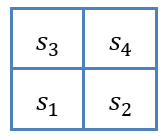
\includegraphics[width=0.15\textwidth]{P1.PNG}
    \caption{$2\times2$的机器人寻路问题}
    \label{fig:my_label}
\end{figure}

\begin{figure}[H]
    \centering
    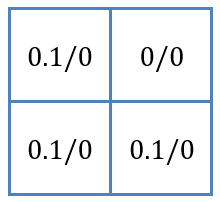
\includegraphics[width=0.15\textwidth]{P2.PNG}
    \caption{Q学习算法的初始状态}
    \label{fig:my_label} 
\end{figure}

\end{problem}


%%%%%%%%%%%%%%%%%%%%%%%%%%%%%%%%%%%%%%%%%%%%%%%%%%%%%%%%%%%%%%%%%%%%%%%%%


\noindent\rule{7in}{1pt}
\textbf{第二部分:实训题(共6分)}
\\ \\
\textbf{实训题要求:}
\begin{itemize}
    \item 本次作业包括1个实训题,作业要求以及基础代码以Aistudio项目的形式发布。
    \item 发布项目链接有效期3天,请在作业发布3天内fork这个项目,生成``我的项目'',并在自己fork的项目下进行作答,生成答案后按要求保存提交。
\end{itemize}

%%%%%%%%%%%%%%%%%%%%%%%%%%%%%%%%%%%%%%%%%%%%%%%%%%%%%%%%%%%%%%%%%%%%%%%%%
% Problem 1
%%%%%%%%%%%%%%%%%%%%%%%%%%%%%%%%%%%%%%%%%%%%%%%%%%%%%%%%%%%%%%%%%%%%%%%%%%%%%%%%%%%%%%%%%%%%%%%%%%%%%%%%%%%%%%%%%%%%%%%%%%%%%%%%%%%%%%%%

\begin{problem}{1 强化学习算法实现 —— CartPole 平衡任务}

本次实验以 OpenAI Gym 中的 CartPole-v1 环境为基础,要求你逐步实现多种强化学习算法,比较不同策略在平衡控制任务中的表现。主要任务如下:

\begin{itemize}
    \item \textbf{任务1:REINFORCE 算法(无基线)} \\
    使用折扣累计回报 $G_t$ 指导策略网络更新,构建基本的策略梯度算法。

    \item \textbf{任务2:REINFORCE + Baseline} \\
    引入基线 $b$,使用优势函数 $A_t = G_t - b$ 减小梯度方差,提升训练稳定性。

    \item \textbf{任务3:Actor-Critic 算法} \\
    结合策略网络(Actor)与价值网络(Critic),分别使用 $A_t = G_t - V(s_t)$ 或 TD 误差 $\delta_t$ 指导训练。

    \item \textbf{任务4:PPO 算法} \\
    通过裁剪概率比值 $r_t$ 的目标函数限制策略更新幅度,提高算法稳定性与性能。

    \item \textbf{任务5:自定义算法优化} \\
    在已有方法基础上,进行个性化设计(如奖励函数、网络结构、归一化等),提出改进策略并验证效果。
\end{itemize}

所有算法需在 CartPole-v1 环境中进行训练与评估,支持可视化 reward 曲线与模型性能分析。
实验介绍详情和参考基础代码请参见Aistudio中的共享项目\href{https://aistudio.baidu.com/studio/project/partial/verify/9223866/1b1108869dd945869c2b33cb1ef240ff}{“人工智能作业四”}。
\end{problem}

\noindent\rule{7in}{1pt}
\textbf{第三部分:实训题实验报告(共3分)}
\begin{itemize}
    \item 请按照实验报告模板完成实验报告。
    \item 实验报告模板是通用模板,可根据每个作业要求的差别,自由进行微调。
\end{itemize}

\end{CJK}
\end{document}